\documentclass[11pt, oneside]{article} 
\usepackage{geometry}
\geometry{letterpaper} 
\usepackage{graphicx}
	
\usepackage{amssymb}
\usepackage{amsmath}
\usepackage{parskip}
\usepackage{color}
\usepackage{hyperref}

\graphicspath{{/Users/telliott/Github/calculus_book/png/}}
% \begin{center} 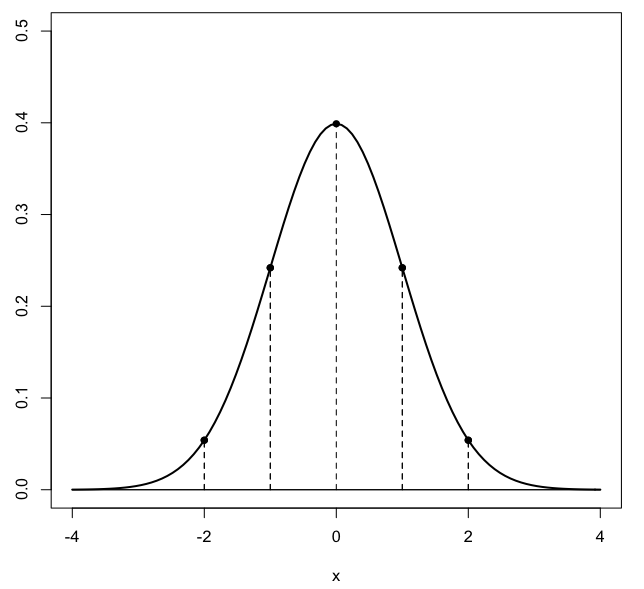
\includegraphics [scale=0.4] {gauss3.png} \end{center}

\title{Irrational numbers}
\date{}

\begin{document}
\maketitle
\Large

\label{sec:general_irrationality}

Theorem:  every integer which is not a perfect square has a square root that is irrational.

A simpler proof based on the fundamental theorem is discussed in the main text and repeated below.

Proof:

Let $D$ be a positive integer but not the square of an integer.

Then, there exists a positive integer $\lambda$ such that
\[ \lambda^2 < D < (\lambda + 1)^2 \]

Now suppose there does exist a rational number $t/u$ whose square is $D$.  We will show that this leads to a contradiction.
\[ \frac{t}{u} = \sqrt{D} \]
\[ t^2 - Du^2 = 0 \]

As previously, we can assume that $u$ is the smallest positive integer with this property since otherwise we could find gcd($t,u$) and divide.

Substituting into the first expression above:
\[ \lambda^2 < (\frac{t}{u})^2 < (\lambda + 1)^2 \]
\[ \lambda < \frac{t}{u} < \lambda + 1 \]
(This last step is justified because $\lambda > 0$ and so are $D$ and $\lambda + 1$).
\[ \lambda u < t < (\lambda + 1)u \]

We next consider two integers.  First, define $v = t - \lambda u$.  By manipulating the left-hand inequality above, we see that $v > 0$.  With the right-hand inequality.
\[ t < (\lambda + 1)u \]
\[ t - \lambda u < u \]

Thus, $v = t - \lambda u$ is also certainly less than $u$ and we have established that
\[ 0 < v < u \]

We then define the integer $s = Du - \lambda t$.  We will show that $Du > \lambda t$ which means that $s > 0$.

From the left-hand inequality
\[ \lambda u < t \]
\[ \lambda < \frac{t}{u} \]
but 
\[ \frac{t}{u} = D \frac{u}{t}  \]
hence
\[ \lambda < D \frac{u}{t} \]
which means that $Du > \lambda t$ as required.

Therefore, we have established that both $s$ and $v$ are positive integers with $v < u$.  

In the next section we will prove that $s$ and $v$ have the same property as $t$ and $u$, namely
\[ s^2 - Dv^2 = 0 \]

This is a contradiction, since we supposed that $u$ was the smallest integer such that $s^2 - Dt^2 = 0$.  Thus, there is no such $u$ and $t$ and $\sqrt{D}$ is irrational.

$\square$

Proof of our lemma:

This is just some messy algebra.  I expand a bit from the answer given in the reference, and work the algebra in reverse.

We defined $s = Du - \lambda t$ so
\[ s^2 = D^2u^2 - 2Du \lambda t + \lambda^2 t^2 \]
and $v = t - \lambda u$ so
\[ Dv^2 = D (t^2 - 2 \lambda ut + \lambda^2 u^2) \]
Subtracting, we obtain:
\[ s^2 - Dv^2 = D^2u^2 - 2Du \lambda t + \lambda^2 t^2 - Dt^2 + 2D \lambda u t - D \lambda^2 u^2 \]
\[ = D^2u^2 + \lambda^2 t^2 - Dt^2 - D \lambda^2 u^2 \]

which factors magically into 
\[ = (\lambda^2 - D)(t^2 - Du^2) \]
but the second term is zero by the definition of $t$ and $u$, so the whole thing is zero, which means that 
\[ s^2 - Dv^2 = 0 \]
as required.

$\square$

\subsection*{much simpler general proof}
We suppose that there exist two integers $a$ and $b$ such that 
\[ (\frac{a}{b})^2 = n \]

According to the fundamental theorem of arithmetic, both $a$ and $b$ have a unique prime factorization.  Suppose that gives $a = a_1 \cdot a_2 \dots a_i$ and likewise for $b$ so:
\[ (\frac{a_1 \cdot a_2 \dots a_i}{b_1 \cdot b_2 \dots b_j})^2 = n \]

If every factor $b$ were some $a_i$, then we could cancel all of them and so $a/b$ would be an integer.

If $a/b$ is to be rational but not an integer, there must be at least one prime factor of $b$ that cannot be cancelled.  Call that (those) $q$, so in lowest terms we have
\[ (\frac{a_1 \cdot a_2 \dots }{q_1 \dots})^2 = n \]

But then, after squaring, we will have $q_1^2$ in the denominator and no corresponding factor of either $q_1$ or $q_1^2$ in the numerator.  Thus, they cannot be canceled and the result cannot be an integer.

This proves that the only $n$ with rational square roots are perfect squares with integer roots.

The proof also applies generally to other powers like cube and the fourth and fifth power and so on.

\end{document}
